\section{Auswertung}
\label{sec:Auswertung}

% \begin{figure}
%   \centering
%   \includegraphics{plots/plot.pdf}
%   \caption{Plot.}
%   \label{fig:plot}
% \end{figure}



% \begin{table}
%    % Notation :  {% nicht entfernen ist sehr wichtig sonst Fehler !!
% \parbox{0.48\textwidth}{% %Ermöglicht zwei Tabellen neben einander
%   \centering
%   \sisetup{round-mode = places , round-precision = 0,scientific-notation=fixed, fixed-exponent = 0}
%          %rundet Werte aus Stelle, Stelle = ,  macht einen bestimmten festen exponenten
%   \resizebox{\textwidth}{!}{%  % skaliert zu große Tabellen
%   \begin{tabular}{S@{${}\pm{}$} S} % fügt plus minus Fehler Schreibweise hinzu
%     \toprule
%      $\text{e}_b / \si{\milli\meter}$ &
%      $\text{d}_b /\si{\milli\meter} $ & $\text{f}_b / \si{\milli\meter} $\\
%     \midrule
%     \bottomrule
%   \end{tabular}
%   % }
%   \caption{Tabellenunterschrift}
%   \label{tab:tab}
% }
% % \end{table}
% % \begin{table}
% \parbox{0.48\textwidth}{%
%   \centering
%   \sisetup{round-mode = places , round-precision = 0,scientific-notation=fixed, fixed-exponent = 0}
%   % \resizebox{\textwidth}{!}{%
%   \begin{tabular}{S@{${}\pm{}$} S}
%     \toprule
%      $\text{e}_b / \si{\milli\meter}$ &
%      $\text{d}_b /\si{\milli\meter} $ & $\text{f}_b / \si{\milli\meter} $\\
%     \midrule
%     \bottomrule
%   \end{tabular}
%   % }
%   \caption{Tabellenunterschrift}
%   \label{tab:tab}
% }
% \end{table}

%%%%%%%%%%%%%%%%%%%%%%%%%%%%%%%%%%%%%%%%%%%%%%%%%%%%%%%%%%%%%%%%%%%%%%%%%%%%%%%%%%%%%%%%%%%%%%%%%%%%
\subsection{Methoden der Auswertung} 
Alle Berechnungen wurden mit dem Paket \cite{numpy} und Fehlerrechnung mit dem Paket 
\cite{uncertainties}  in der Programmiersprache \textit{Python} durchgeführt. 
Physikalische Konstanten wurden aus dem Paket \cite{scipy} entnommen. Die Diagramme wurden 
mit dem Paket \cite{matplotlib} erzeugt.

\subsection{Bestimmung von \texorpdfstring{$C_p \text{ und } C_V$}{math}}
Zuerst wird $C_p$ bestimmt. Der Zusammenhang zur Molwärme ist über die elektrisch erzeugte 
Wärmeenergie in der Probe gegeben. Daraus folgt die Gleichung
\begin{equation}
C_p = \frac{U\cdot I \cdot t_H \cdot M}{\Delta T \cdot m} \; .
\label{eq:Cp}
\end{equation} 
Hier bei ist $U$ die an der Probe angelegte Spannung, $I$ der angelegte Strom, $t_H$ die Heizdauer, 
$M$ die Molmasse, $m$ die Masse der Probe und $\Delta T$ die Temperaturänderung. 
Die fehlerbehafteten Größen sind hier bei $U$ und $I$ mit \SI{10}{\percent} der Skala,
$t_H$ mit $\pm 5\;\si{\second}$ und $\Delta T$ mit \SI{0.2}{\percent} auf den gemessenen Widerstand 
der Pt-100-Widstände, die linear mit der Temperatur zusammenhängen. Der Fehler der 
Gleichung \eqref{eq:Cp} ist dann durch Gauß'sche Fehlerfortpflanzung gegeben;
\begin{equation}
\sigma(C_{p} )= \sqrt{\left(\frac{I t_H  M }{\Delta T  m} \sigma(U) \right)^2 + 
\left(\frac{U t_H  M}{\Delta T  m} \sigma(I) \right)^2 + 
\left(\frac{U  I  M}{\Delta T  m}\sigma(t_H) \right)^2 + 
\left(-\frac{U  I  t_H  M }{ \Delta T^2  m } \sigma(\Delta T) \right)^2 } \; .
\end{equation}
Zur Berechnung wurde die Masse der Probe $m = \SI{0.342}{\kilo\gram}$ aus der Quelle 
\cite{Anleitung} entnommen, die Molmasse wurde mit \SI{0.0635}{\kilo\gram\per\mol} aus Quelle 
\cite{Kupfer} entnommen, genauso wie das Kompressionsmodul $\kappa = \SI{137,8}{\giga\pascal}$ und 
die Dichte $\rho = \SI{8960}{\kilo\gram\per\cubic\meter}$, die später gebraucht werden. Ist $C_p$ 
berechnet, kann mit der Gleichung
\begin{equation}
C_p - C_V = 9\cdot \alpha^2 \cdot  \kappa \cdot V_0 \cdot T 
\quad \iff \quad 
C_V = C_p - 9\cdot \alpha^2 \cdot \kappa \cdot V_0 \cdot T  
\label{eq:Cv}
\end{equation}
$C_V$ berechnet werden.  Dabei bezeichnet $\kappa$ das zuvor erwähnte Kompressionsmodul, $T$ die 
Temperatur und $\alpha$ den temperaturabhängigen Ausdehnungskoeffizient, 
der aus der Quelle \cite{Anleitung} entnommen 
wurde. Das Molvolumen $V_0$ ist durch $\frac{M}{\rho} = \SI{7.09e-6}{\mol\per\cubic\meter}$ 
gegeben. Der Fehler ist durch 
\begin{equation}
\sigma(C_V) = \sqrt{\left(\sigma(C_p) \right)^2 + \left( -9\alpha^2 \kappa V_0 \sigma(T)\right)^2
+ \left(-18 \alpha \kappa V_0 T \sigma(\alpha) \right)^2}
\end{equation} 
gegeben. Alle Werte dazu wurden in den Tabellen \ref{tab:CP} und \ref{tab:CV} festgehalten. 
Die Ergebnisse sind in der Abbildung \ref{fig:CVP1} und \ref{fig:CVP2} festgehalten. 

\begin{figure}
  \centering
  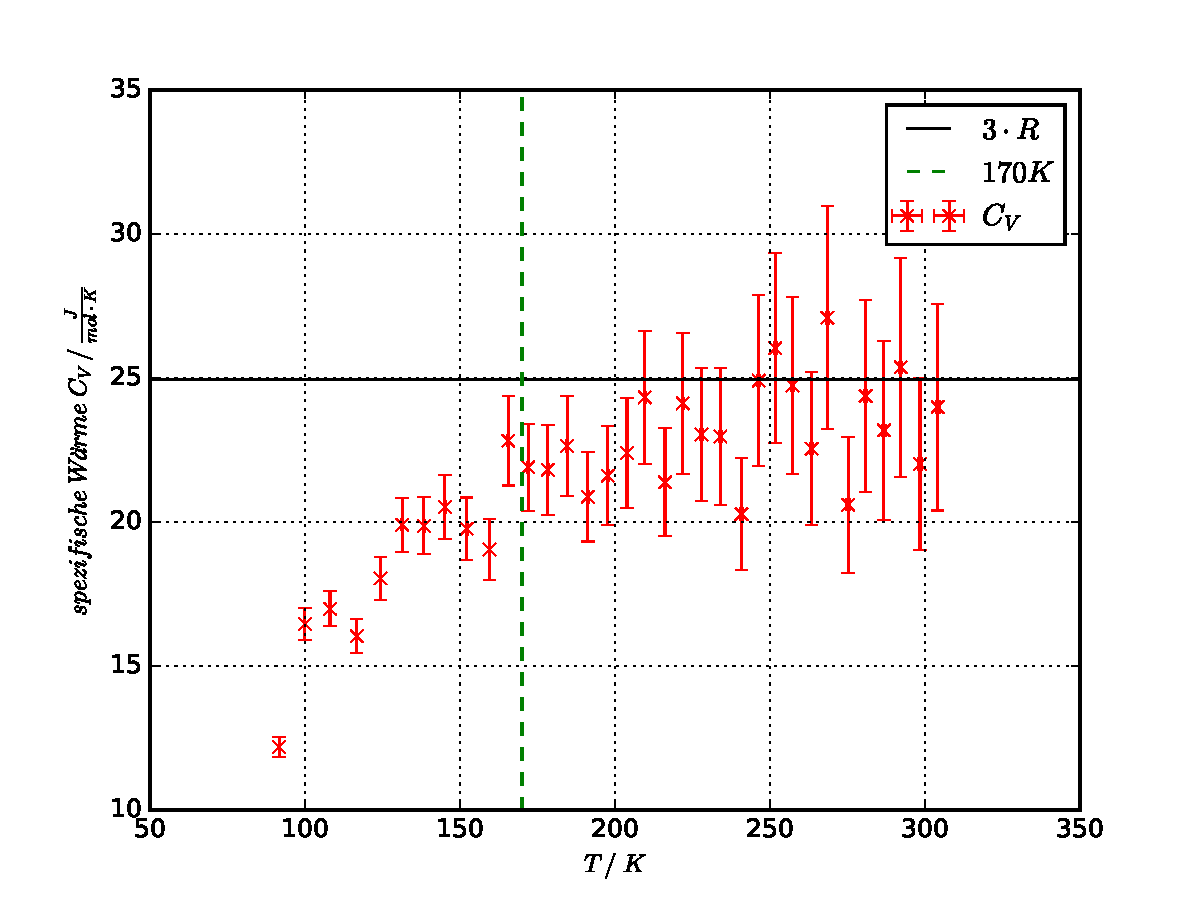
\includegraphics[height = 12cm]{plots/Cplot1.pdf}
  \caption{Die spezifischen Wärmekapazitäten \texorpdfstring{$C_V$}{math} in Abhängigkeit von der Temperatur dargestellt.}
  \label{fig:CVP1}
\end{figure}
\begin{figure}
  \centering
  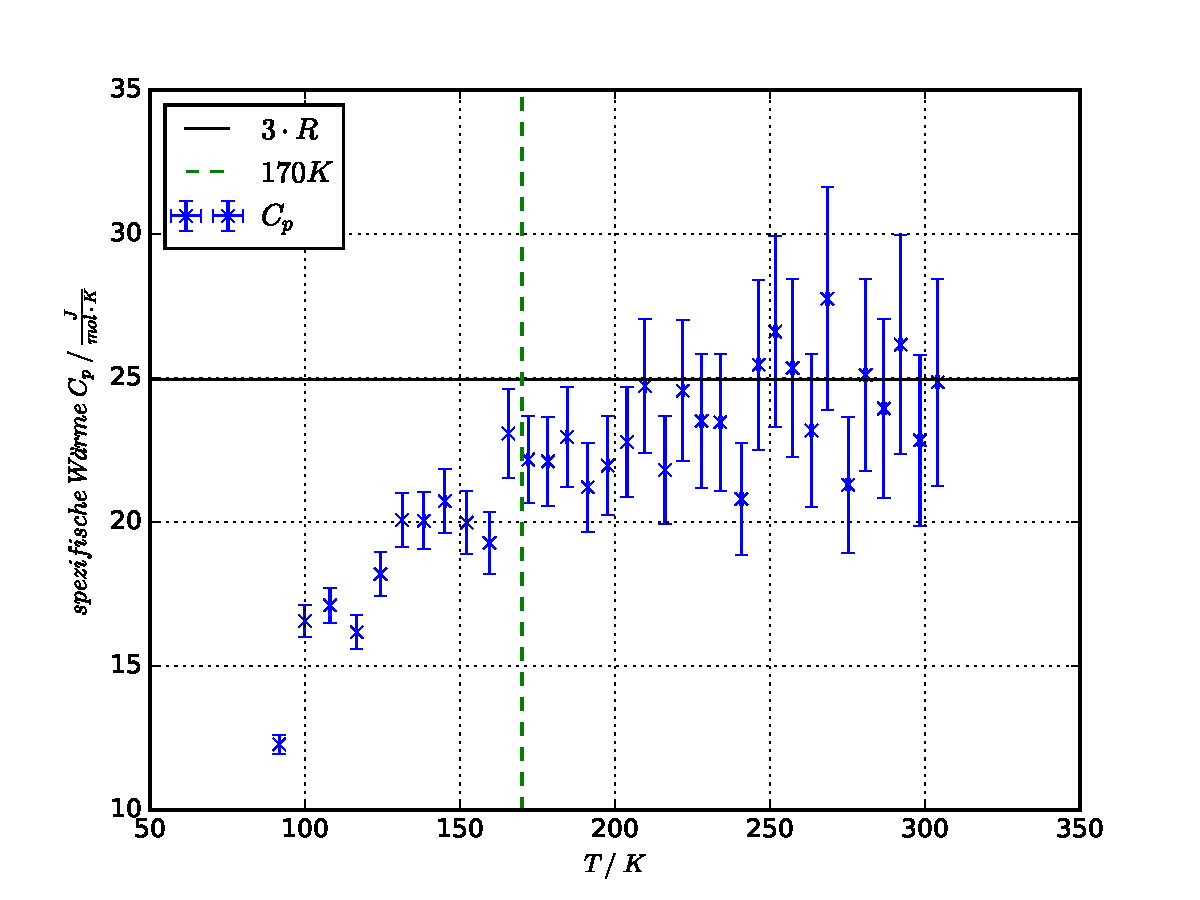
\includegraphics[height = 12cm]{plots/Cplot2.pdf}
  \caption{Die spezifischen Wärmekapazitäten \texorpdfstring{$C_p$}{math} in Abhängigkeit von der Temperatur dargestellt.}
  \label{fig:CVP2}
\end{figure}


\begin{table}
  \centering
  %\sisetup{round-mode = places , round-precision = 0,scientific-notation=fixed, fixed-exponent = 0}
  \resizebox{\textwidth}{!}{%
  \begin{tabular}{  
|S[round-mode = places , round-precision = 1,scientific-notation=fixed, fixed-exponent = 0]
@{${}\pm{}$} 
S[round-mode = places , round-precision = 1,scientific-notation=fixed, fixed-exponent = 0] 
|S[round-mode = places , round-precision = 2,scientific-notation=fixed, fixed-exponent = 0]
@{$\quad\pm{}$} 
S[round-mode = places , round-precision = 0,scientific-notation=true]%, fixed-exponent = 0] 
|S[round-mode = places , round-precision = 1,scientific-notation=fixed, fixed-exponent = -3]
@{$\qquad\pm{}$} 
S[round-mode = places , round-precision = 1,scientific-notation=fixed, fixed-exponent = -4] 
|S[round-mode = places , round-precision = 0,scientific-notation=fixed, fixed-exponent = 0]
@{${}\pm \quad$} 
S[round-mode = places , round-precision = 0,scientific-notation=fixed, fixed-exponent = 0]
|S[round-mode = places , round-precision = 0,scientific-notation=fixed, fixed-exponent = 0]
@{${}\pm{}$} 
S[round-mode = places , round-precision = 0,scientific-notation=true]|
}
    \toprule
     \multicolumn{2}{c}{$\Delta T  / \si{\kelvin}$} & 
    \multicolumn{2}{c}{$U /\si{\volt}$}  & \multicolumn{2}{c}{$I / \si{\ampere} $} & 
     \multicolumn{2}{c}{$t_H / \si{\second}$} & 
    \multicolumn{2}{c}{$ C_p / \si{\joule\per\mol\kelvin}$} \\ 
    \midrule
1.109413379999998028e+01 & 1.614153408060262918e-01 & 1.601000000000000156e+01 & 1.000000000000000021e-03 & 1.525999999999999857e-01 & 1.000000000000000082e-05 & 3.000000000000000000e+02 & 7.071067811865475505e+00 & 1.227540509995699658e+01 & 3.400209563735166474e-01\\
8.300047000000006392e+00 & 1.892259528562504067e-01 & 1.610000000000000142e+01 & 1.000000000000000021e-03 & 1.532000000000000028e-01 & 1.000000000000000082e-05 & 3.000000000000000000e+02 & 7.071067811865475505e+00 & 1.656484805909121150e+01 & 5.431958493109000363e-01\\
8.094339200000007395e+00 & 2.131336659919116638e-01 & 1.616000000000000014e+01 & 1.000000000000000021e-03 & 1.537000000000000033e-01 & 1.000000000000000082e-05 & 3.000000000000000000e+02 & 7.071067811865475505e+00 & 1.710476811747318493e+01 & 6.044776947283907464e-01\\
8.604244800000003579e+00 & 2.376420091583867633e-01 & 1.621000000000000085e+01 & 1.000000000000000021e-03 & 1.539999999999999980e-01 & 1.000000000000000082e-05 & 3.000000000000000000e+02 & 7.071067811865475505e+00 & 1.617239516672464106e+01 & 5.872119735496813542e-01\\
7.677376000000009526e+00 & 2.615220766611146552e-01 & 1.625000000000000000e+01 & 1.000000000000000021e-03 & 1.542000000000000037e-01 & 1.000000000000000082e-05 & 3.000000000000000000e+02 & 7.071067811865475505e+00 & 1.819316654899107633e+01 & 7.536274376786966656e-01\\
6.981326599999988503e+00 & 2.831194473254090016e-01 & 1.628000000000000114e+01 & 1.000000000000000021e-03 & 1.544000000000000095e-01 & 1.000000000000000082e-05 & 3.000000000000000000e+02 & 7.071067811865475505e+00 & 2.006998777292535152e+01 & 9.414034519191893935e-01\\
7.003865399999995134e+00 & 3.038320614411661458e-01 & 1.630000000000000071e+01 & 1.000000000000000021e-03 & 1.544999999999999984e-01 & 1.000000000000000082e-05 & 3.000000000000000000e+02 & 7.071067811865475505e+00 & 2.004295096153079925e+01 & 9.895296783345467473e-01\\
6.783739200000013625e+00 & 3.243005555873718637e-01 & 1.630999999999999872e+01 & 1.000000000000000021e-03 & 1.545999999999999874e-01 & 1.000000000000000082e-05 & 3.000000000000000000e+02 & 7.071067811865475505e+00 & 2.071942383628665141e+01 & 1.104354335199625003e+00\\
7.048165799999992487e+00 & 3.449182479580759630e-01 & 1.632999999999999829e+01 & 1.000000000000000021e-03 & 1.547000000000000042e-01 & 1.000000000000000082e-05 & 3.000000000000000000e+02 & 7.071067811865475505e+00 & 1.997946034795793935e+01 & 1.085240336079606571e+00\\
7.314923999999990656e+00 & 3.663888896618556212e-01 & 1.633999999999999986e+01 & 1.000000000000000021e-03 & 1.548000000000000209e-01 & 1.000000000000000082e-05 & 3.000000000000000000e+02 & 7.071067811865475505e+00 & 1.927509633233781017e+01 & 1.067004500271659717e+00\\
6.114194999999995161e+00 & 3.864588135510672595e-01 & 1.635000000000000142e+01 & 1.000000000000000021e-03 & 1.548000000000000209e-01 & 1.000000000000000082e-05 & 3.000000000000000000e+02 & 7.071067811865475505e+00 & 2.307452633464501801e+01 & 1.556575696886436377e+00\\
6.376531200000016497e+00 & 4.052326649010017934e-01 & 1.637000000000000099e+01 & 1.000000000000000021e-03 & 1.549000000000000099e-01 & 1.000000000000000082e-05 & 3.000000000000000000e+02 & 7.071067811865475505e+00 & 2.216659442155588522e+01 & 1.502471297299011965e+00\\
6.394647999999989452e+00 & 4.244664500271059793e-01 & 1.637000000000000099e+01 & 1.000000000000000021e-03 & 1.549000000000000099e-01 & 1.000000000000000082e-05 & 3.000000000000000000e+02 & 7.071067811865475505e+00 & 2.210379381739192794e+01 & 1.556969387638461821e+00\\
6.165784999999971205e+00 & 4.434212576054418764e-01 & 1.637999999999999901e+01 & 1.000000000000000021e-03 & 1.549999999999999989e-01 & 1.000000000000000082e-05 & 3.000000000000000000e+02 & 7.071067811865475505e+00 & 2.295305966981107204e+01 & 1.737098813160012245e+00\\
6.677861400000040248e+00 & 4.628766607253544385e-01 & 1.639000000000000057e+01 & 1.000000000000000021e-03 & 1.549999999999999989e-01 & 1.000000000000000082e-05 & 3.000000000000000000e+02 & 7.071067811865475505e+00 & 2.120589554005422173e+01 & 1.552547777926402972e+00\\
6.448998399999965159e+00 & 4.827845240598436782e-01 & 1.639000000000000057e+01 & 1.000000000000000021e-03 & 1.549999999999999989e-01 & 1.000000000000000082e-05 & 3.000000000000000000e+02 & 7.071067811865475505e+00 & 2.195845346765194606e+01 & 1.723406157996266730e+00\\
6.218045000000017808e+00 & 5.020423374234488367e-01 & 1.639000000000000057e+01 & 1.000000000000000021e-03 & 1.549999999999999989e-01 & 1.000000000000000082e-05 & 3.000000000000000000e+02 & 7.071067811865475505e+00 & 2.277404413756424617e+01 & 1.915518219660888422e+00\\
5.735395000000039545e+00 & 5.202503424681603761e-01 & 1.639999999999999858e+01 & 1.000000000000000021e-03 & 1.550999999999999879e-01 & 1.000000000000000082e-05 & 3.000000000000000000e+02 & 7.071067811865475505e+00 & 2.472154901189958309e+01 & 2.316929558272094791e+00\\
6.500561599999969076e+00 & 5.389664746571235510e-01 & 1.639000000000000057e+01 & 1.000000000000000021e-03 & 1.550999999999999879e-01 & 1.000000000000000082e-05 & 3.000000000000000000e+02 & 7.071067811865475505e+00 & 2.179833086880748283e+01 & 1.878929740359342127e+00\\
5.765598599999975704e+00 & 5.577282552787762304e-01 & 1.639000000000000057e+01 & 1.000000000000000021e-03 & 1.549999999999999989e-01 & 1.000000000000000082e-05 & 3.000000000000000000e+02 & 7.071067811865475505e+00 & 2.456120189833570677e+01 & 2.445411652128524516e+00\\
6.031392000000039388e+00 & 5.758386336485257218e-01 & 1.639999999999999858e+01 & 1.000000000000000021e-03 & 1.550999999999999879e-01 & 1.000000000000000082e-05 & 3.000000000000000000e+02 & 7.071067811865475505e+00 & 2.350831260762090480e+01 & 2.311809110967832925e+00\\
6.046828799999957482e+00 & 5.944135881562774282e-01 & 1.639999999999999858e+01 & 1.000000000000000021e-03 & 1.552000000000000046e-01 & 1.000000000000000082e-05 & 3.000000000000000000e+02 & 7.071067811865475505e+00 & 2.346341699763582866e+01 & 2.371870492070308867e+00\\
6.821134199999988823e+00 & 6.142670873678979238e-01 & 1.639999999999999858e+01 & 1.000000000000000021e-03 & 1.552000000000000046e-01 & 1.000000000000000082e-05 & 3.000000000000000000e+02 & 7.071067811865475505e+00 & 2.079995224954129895e+01 & 1.936206137786079751e+00\\
5.572406400000033955e+00 & 6.333792794191224207e-01 & 1.639999999999999858e+01 & 1.000000000000000021e-03 & 1.552000000000000046e-01 & 1.000000000000000082e-05 & 3.000000000000000000e+02 & 7.071067811865475505e+00 & 2.546104061033883070e+01 & 2.955560462919106346e+00\\
5.331215399999990723e+00 & 6.502509702422637483e-01 & 1.639999999999999858e+01 & 1.000000000000000021e-03 & 1.552000000000000046e-01 & 1.000000000000000082e-05 & 3.000000000000000000e+02 & 7.071067811865475505e+00 & 2.661293063636354361e+01 & 3.306046359520455447e+00\\
5.597759199999984503e+00 & 6.672046495557519830e-01 & 1.639999999999999858e+01 & 1.000000000000000021e-03 & 1.552000000000000046e-01 & 1.000000000000000082e-05 & 3.000000000000000000e+02 & 7.071067811865475505e+00 & 2.534572506222012223e+01 & 3.079495032234256247e+00\\
6.121440000000006876e+00 & 6.854247387305468786e-01 & 1.639999999999999858e+01 & 1.000000000000000021e-03 & 1.552000000000000046e-01 & 1.000000000000000082e-05 & 3.000000000000000000e+02 & 7.071067811865475505e+00 & 2.317743303008976596e+01 & 2.652080155581815646e+00\\
5.112992000000019743e+00 & 7.028925881256223862e-01 & 1.639999999999999858e+01 & 1.000000000000000021e-03 & 1.552000000000000046e-01 & 1.000000000000000082e-05 & 3.000000000000000000e+02 & 7.071067811865475505e+00 & 2.774877520788460572e+01 & 3.870340373341230045e+00\\
6.662915999999995620e+00 & 7.212933952059549236e-01 & 1.639000000000000057e+01 & 1.000000000000000021e-03 & 1.553000000000000214e-01 & 1.000000000000000082e-05 & 3.000000000000000000e+02 & 7.071067811865475505e+00 & 2.129459762225272357e+01 & 2.359253997447231299e+00\\
5.652002399999958016e+00 & 7.405172514765353542e-01 & 1.639000000000000057e+01 & 1.000000000000000021e-03 & 1.553000000000000214e-01 & 1.000000000000000082e-05 & 3.000000000000000000e+02 & 7.071067811865475505e+00 & 2.510333598069077254e+01 & 3.341802640667225432e+00\\
5.922780600000010054e+00 & 7.586480361827677710e-01 & 1.637999999999999901e+01 & 1.000000000000000021e-03 & 1.553000000000000214e-01 & 1.000000000000000082e-05 & 3.000000000000000000e+02 & 7.071067811865475505e+00 & 2.394104345540300471e+01 & 3.118091946768671630e+00\\
5.420137800000020434e+00 & 7.764335509412996217e-01 & 1.637999999999999901e+01 & 1.000000000000000021e-03 & 1.553000000000000214e-01 & 1.000000000000000082e-05 & 3.000000000000000000e+02 & 7.071067811865475505e+00 & 2.616124404095733524e+01 & 3.797984053907824453e+00\\
6.208915199999978540e+00 & 7.947272077303743076e-01 & 1.637999999999999901e+01 & 1.000000000000000021e-03 & 1.553000000000000214e-01 & 1.000000000000000082e-05 & 3.000000000000000000e+02 & 7.071067811865475505e+00 & 2.283773302644214453e+01 & 2.972327993274054947e+00\\
5.705066400000077920e+00 & 8.134783488621806224e-01 & 1.637999999999999901e+01 & 1.000000000000000021e-03 & 1.553000000000000214e-01 & 1.000000000000000082e-05 & 3.000000000000000000e+02 & 7.071067811865475505e+00 & 2.485467088015245452e+01 & 3.592090571804302801e+00\\
    \bottomrule
  \end{tabular}
  }
  \caption{Temperaturunterschied \texorpdfstring{$\Delta T$}{math} der Probe in Zeitraum 
	\texorpdfstring{$t_H$}{math} in dem die Spannung und Strom 
	\texorpdfstring{$U \; , \; I$}{math} angelegt ist. Und die daraus resultierende 
	Molwärme \texorpdfstring{$C_p$}{math}. }
  \label{tab:CP}
\end{table}

\begin{table}
  \centering
  %\sisetup{round-mode = places , round-precision = 0,scientific-notation=fixed, fixed-exponent = 0}
%  \resizebox{\textwidth}{!}{%
  \begin{tabular}{  
|S[round-mode = places , round-precision = 1,scientific-notation=fixed, fixed-exponent = 0]
@{${}\pm \quad$} 
S[round-mode = places , round-precision = 1,scientific-notation=fixed, fixed-exponent = 0]
|S[round-mode = places , round-precision = 0,scientific-notation=fixed, fixed-exponent = 0]
@{${}\pm{}$} 
S[round-mode = places , round-precision = 0] 
|S[round-mode = places , round-precision = 1,scientific-notation=fixed, fixed-exponent = -6 ] 
@{$\quad\pm{}$}
S[round-mode = places , round-precision = 0]
|S[round-mode = places , round-precision = 0,scientific-notation=fixed, fixed-exponent = 0]
@{${}\pm{}$} 
S[round-mode = places , round-precision = 0] |
}
    \toprule
     \multicolumn{2}{c}{$ T  / \si{\kelvin}$} & 
    \multicolumn{2}{c}{$C_p / \si{\joule\per\mol\kelvin}$}& 
    \multicolumn{2}{c}{$\alpha_T / \si{\kelvin}$} & 
    \multicolumn{2}{c}{$C_V / \si{\joule\per\mol\kelvin}$}\\
    \midrule
9.167832639999994626e+01 & 1.249645055999999699e-01 & 1.227540509995699658e+01 & 3.400209563735166474e-01 & 1.052256786563874041e-05 & 3.371115694249032316e-07 & 1.219692396672422596e+01 & 3.400581531192610196e-01\\
9.997837339999995265e+01 & 1.420926935999999863e-01 & 1.656484805909121150e+01 & 5.431958493109000363e-01 & 1.081332212074735926e-05 & 3.181061725486583042e-07 & 1.647055995716445409e+01 & 5.432241916021363082e-01\\
1.080727125999999600e+02 & 1.588572503999999552e-01 & 1.710476811747318493e+01 & 6.044776947283907464e-01 & 1.109687034218423453e-05 & 3.002749807420602475e-07 & 1.699648044334717767e+01 & 6.045061219384838536e-01\\
1.166769573999999636e+02 & 1.767430296000000178e-01 & 1.617239516672464106e+01 & 5.872119735496813542e-01 & 1.139828077848612421e-05 & 2.822304053626104042e-07 & 1.604889524287808200e+01 & 5.872438498597467582e-01\\
1.243543333999999732e+02 & 1.927581335999999923e-01 & 1.819316654899107633e+01 & 7.536274376786966656e-01 & 1.166722259773953218e-05 & 2.670729153948287462e-07 & 1.805346796671719645e+01 & 7.536546051608478125e-01\\
1.313356599999999617e+02 & 2.073666399999999910e-01 & 2.006998777292535152e+01 & 9.414034519191893935e-01 & 1.191178150388222924e-05 & 2.542019133002215546e-07 & 1.991478970988911001e+01 & 9.414267863957349602e-01\\
1.383395253999999568e+02 & 2.220653015999999869e-01 & 2.004295096153079925e+01 & 9.895296783345467473e-01 & 1.215712995398835675e-05 & 2.423067309517869946e-07 & 1.987221825901713856e+01 & 9.895531194950224485e-01\\
1.451232645999999704e+02 & 2.363426584000000163e-01 & 2.071942383628665141e+01 & 1.104354335199625003e+00 & 1.239476728760190577e-05 & 2.319047907116195273e-07 & 2.053248696418650354e+01 & 1.104376529848418054e+00\\
1.521714303999999629e+02 & 2.512185216000000221e-01 & 1.997946034795793935e+01 & 1.085240336079606571e+00 & 1.264166759998098307e-05 & 2.224317736158506170e-07 & 1.977546620007873202e+01 & 1.085264129056846993e+00\\
1.594863543999999536e+02 & 2.667022176000000133e-01 & 1.927509633233781017e+01 & 1.067004500271659717e+00 & 1.289791256808732704e-05 & 2.142286672113401882e-07 & 1.905243545503550351e+01 & 1.067030200320947975e+00\\
1.656005493999999487e+02 & 2.796789975999999789e-01 & 2.307452633464501801e+01 & 1.556575696886436377e+00 & 1.311209547727010843e-05 & 2.087856444635466220e-07 & 2.283334723339878636e+01 & 1.556594698450650904e+00\\
1.719770805999999652e+02 & 2.932459223999999698e-01 & 2.216659442155588522e+01 & 1.502471297299011965e+00 & 1.333546813759755844e-05 & 2.045995594802491861e-07 & 2.190756431686457972e+01 & 1.502492384926692015e+00\\
1.783717285999999547e+02 & 3.068853143999999977e-01 & 2.210379381739192794e+01 & 1.556969387638461821e+00 & 1.355947543730583743e-05 & 2.020232957634908221e-07 & 2.182567633754424818e+01 & 1.556991515544013716e+00\\
1.845375135999999259e+02 & 3.200684543999999243e-01 & 2.295305966981107204e+01 & 1.737098813160012245e+00 & 1.377546556661894762e-05 & 2.011357584514392366e-07 & 2.265533794400208834e+01 & 1.737120645219006443e+00\\
1.912153749999999661e+02 & 3.343815000000000537e-01 & 2.120589554005422173e+01 & 1.552547777926402972e+00 & 1.400939395486489259e-05 & 2.019663753588234130e-07 & 2.088733256635079982e+01 & 1.552575046343992682e+00\\
1.976643733999999313e+02 & 3.482382935999999152e-01 & 2.195845346765194606e+01 & 1.723406157996266730e+00 & 1.423530517271566536e-05 & 2.045159016118897599e-07 & 2.161763092748586601e+01 & 1.723434084827526247e+00\\
2.038824183999999491e+02 & 3.616304736000000020e-01 & 2.277404413756424617e+01 & 1.915518219660888422e+00 & 1.445312599255040455e-05 & 2.085410153498657041e-07 & 2.241086247459758951e+01 & 1.915546997841493626e+00\\
2.096178133999999886e+02 & 3.740104536000000701e-01 & 2.472154901189958309e+01 & 2.316929558272094791e+00 & 1.465403937303833523e-05 & 2.135423161485327087e-07 & 2.433645530614702324e+01 & 2.316956842159153318e+00\\
2.161183749999999577e+02 & 3.880734999999999602e-01 & 2.179833086880748283e+01 & 1.878929740359342127e+00 & 1.488175687220378153e-05 & 2.205965434753570968e-07 & 2.139000346054177371e+01 & 1.878968877691187256e+00\\
2.218839735999999334e+02 & 4.005742943999999750e-01 & 2.456120189833570677e+01 & 2.445411652128524516e+00 & 1.508372829793164619e-05 & 2.279797040731864712e-07 & 2.412870695826712364e+01 & 2.445446722608912715e+00\\
2.279153655999999728e+02 & 4.136790624000000749e-01 & 2.350831260762090480e+01 & 2.311809110967832925e+00 & 1.529501058202329991e-05 & 2.367247594343931408e-07 & 2.305175305491104609e+01 & 2.311852455204410184e+00\\
2.339621943999999303e+02 & 4.268455775999998592e-01 & 2.346341699763582866e+01 & 2.371870492070308867e+00 & 1.550683362393057328e-05 & 2.464305486163195356e-07 & 2.298136732124601522e+01 & 2.371920137002112572e+00\\
2.407833285999999191e+02 & 4.417317144000000306e-01 & 2.079995224954129895e+01 & 1.936206137786079751e+00 & 1.574578092065273747e-05 & 2.583741160058937664e-07 & 2.028974569819172302e+01 & 1.936278760422485590e+00\\
2.463557349999999531e+02 & 4.539189399999999930e-01 & 2.546104061033883070e+01 & 2.955560462919106346e+00 & 1.594098473961840027e-05 & 2.688201730763348077e-07 & 2.492285926303315691e+01 & 2.955616363950850367e+00\\
2.516869503999999438e+02 & 4.656006015999999414e-01 & 2.661293063636354361e+01 & 3.306046359520455447e+00 & 1.612773953298891734e-05 & 2.793253022003739603e-07 & 2.604931684156714766e+01 & 3.306104166610511097e+00\\
2.572847095999999283e+02 & 4.778892383999999161e-01 & 2.534572506222012223e+01 & 3.079495032234256247e+00 & 1.632383147156148270e-05 & 2.908335255058934383e-07 & 2.475582717713562886e+01 & 3.079566962685963194e+00\\
2.634061495999999352e+02 & 4.913541983999999974e-01 & 2.317743303008976596e+01 & 2.652080155581815646e+00 & 1.653826817624425241e-05 & 3.039140082445202073e-07 & 2.255846820058305013e+01 & 2.652177968563707466e+00\\
2.685191415999999549e+02 & 5.026221663999999034e-01 & 2.774877520788460572e+01 & 3.870340373341230045e+00 & 1.671737850903348924e-05 & 3.151912281600877577e-07 & 2.710128352075066971e+01 & 3.870417573517058507e+00\\
2.751820575999999505e+02 & 5.173346304000000506e-01 & 2.129459762225272357e+01 & 2.359253997447231299e+00 & 1.695078335341946644e-05 & 3.303098220928112403e-07 & 2.061597750124116502e+01 & 2.359402577049205529e+00\\
2.808340599999999085e+02 & 5.298402400000000734e-01 & 2.510333598069077254e+01 & 3.341802640667225432e+00 & 1.714877545487191468e-05 & 3.434664967384489739e-07 & 2.439153550021916317e+01 & 3.341924544089816429e+00\\
2.867568405999999186e+02 & 5.429697624000000555e-01 & 2.394104345540300471e+01 & 3.118091946768671630e+00 & 1.735625303439945126e-05 & 3.575416122930851342e-07 & 2.319693941917595126e+01 & 3.118242971776192807e+00\\
2.921769783999999390e+02 & 5.550071135999999905e-01 & 2.616124404095733524e+01 & 3.797984053907824453e+00 & 1.754612281810369716e-05 & 3.706524751575589065e-07 & 2.538473225400489142e+01 & 3.798126027565813967e+00\\
2.983858935999999176e+02 & 5.688219743999999300e-01 & 2.283773302644214453e+01 & 2.972327993274054947e+00 & 1.776362381707497423e-05 & 3.859119802142150842e-07 & 2.202680732704448019e+01 & 2.972537222705113891e+00\\
3.040909599999999955e+02 & 5.815398399999999191e-01 & 2.485467088015245452e+01 & 3.592090571804302801e+00 & 1.796347477351862293e-05 & 4.001356109712336449e-07 & 2.400777324488833031e+01 & 3.592289071918686627e+00\\
    \bottomrule
  \end{tabular}
%  }
  \caption{Die Molwärme \texorpdfstring{$C_p$}{math}, Temperatur T, 
	 temperaturabhängiger Ausdehnungskoeffizient \texorpdfstring{$\alpha_T$}{math}  
	und die daraus resultierende Molwärme \texorpdfstring{$C_V$}{math}.}
  \label{tab:CV}
\end{table}

\FloatBarrier

\subsection{Bestimmung der Debye-Temperatur \texorpdfstring{$\theta_D$}{math}}
\label{sec:DT1}
Zur Bestimmung der Debye-Temperatur werden die Molwärmen $C_V$ unter \SI{170}{\kelvin} betrachtet. 
Die Quotienten $\frac{\theta_D}{T}$ können dann für ein gegebenes $C_V$ aus der Debye-Funktion 
aus Quelle \cite{Anleitung} ausgelesen werden. Die Werte dazu sind in der Tabelle \ref{tab:theta} 
dargestellt. Durch einfache Multiplikation kann dann die Debye-Temperatur bestimmt werden.

\begin{table}
  \centering
  %\sisetup{round-mode = places , round-precision = 0,scientific-notation=fixed, fixed-exponent = 0}
  \begin{tabular}{S[round-mode = places , round-precision = 1,scientific-notation=fixed, fixed-exponent = 0]@{${}\pm{}$} S[round-mode = places , round-precision = 0] S[round-mode = places , round-precision = 1,scientific-notation=fixed, fixed-exponent = 0] S[round-mode = places , round-precision = 1,scientific-notation=fixed, fixed-exponent = 0]@{${}\pm{}$} S[round-mode = places , round-precision = 1,scientific-notation=fixed, fixed-exponent = 0] S[round-mode = places , round-precision = 0,scientific-notation=fixed, fixed-exponent = 0]@{${}\pm{}$} S[round-mode = places , round-precision = 1,scientific-notation=fixed, fixed-exponent = 0]}
    \toprule
	\multicolumn{2}{c}{$C_V / \si{\joule\per\mol\kelvin}$} &
	$ \frac{\theta_D}{T}  $ &
	\multicolumn{2}{c}{$T / \si{\kelvin}$} &
	\multicolumn{2}{c}{$\theta_D / \si{\kelvin}$} \\
    \midrule
	1.219425494565318679e+01 & 3.400209719400973940e-01 & 4.099999999999999645e+00 & 9.167832639999994626e+01 & 1.249645055999999699e-01 & 3.758811382399997569e+02 & 5.123544729600000291e-01\\
	1.647252585428109484e+01 & 5.431958638878240375e-01 & 3.000000000000000000e+00 & 9.997837339999995265e+01 & 1.420926935999999863e-01 & 2.999351201999998580e+02 & 4.262780808000000143e-01\\
	1.698846973268172178e+01 & 6.044777173263095049e-01 & 2.899999999999999911e+00 & 1.080727125999999600e+02 & 1.588572503999999552e-01 & 3.134108665399998586e+02 & 4.606860261599999840e-01\\
	1.603322096832429722e+01 & 5.872120091844975631e-01 & 3.100000000000000089e+00 & 1.166769573999999636e+02 & 1.767430296000000178e-01 & 3.616985679399999185e+02 & 5.479033917599999137e-01\\
	1.802894199837958666e+01 & 7.536274787372699846e-01 & 2.600000000000000089e+00 & 1.243543333999999732e+02 & 1.927581335999999923e-01 & 3.233212668399999643e+02 & 5.011711473600000133e-01\\
	1.988084734593920899e+01 & 9.414034975718943432e-01 & 2.200000000000000178e+00 & 1.313356599999999617e+02 & 2.073666399999999910e-01 & 2.889384519999999270e+02 & 4.562066079999999579e-01\\
	1.984319207792999151e+01 & 9.895297285995637848e-01 & 2.200000000000000178e+00 & 1.383395253999999568e+02 & 2.220653015999999869e-01 & 3.043469558799999390e+02 & 4.885436635199998934e-01\\
	2.049436501819791090e+01 & 1.104354394290778085e+00 & 2.000000000000000000e+00 & 1.451232645999999704e+02 & 2.363426584000000163e-01 & 2.902465291999999408e+02 & 4.726853168000000327e-01\\
	1.973283450901056923e+01 & 1.085240410403998768e+00 & 2.200000000000000178e+00 & 1.521714303999999629e+02 & 2.512185216000000221e-01 & 3.347771468799999184e+02 & 5.526807475199999597e-01\\
	1.901649267709574787e+01 & 1.067004585681934570e+00 & 2.399999999999999911e+00 & 1.594863543999999536e+02 & 2.667022176000000133e-01 & 3.827672505599998658e+02 & 6.400853222400000320e-01\\
	2.278967045029140337e+01 & 1.556575769774486195e+00 & 1.399999999999999911e+00 & 1.656005493999999487e+02 & 2.796789975999999789e-01 & 2.318407691599999225e+02 & 3.915505966399999704e-01\\
    \bottomrule
  \end{tabular}
  \caption{Die Molwärme \texorpdfstring{$C_V$}{math}, Temperatur T, der Quotient aus der Debye-Temperatur \texorpdfstring{$\theta_D$}{math} und der Temperatur, sowie die Debye-Temperatur berechnet aus dem Quotienten multipliziert mit der Temperatur.}
  \label{tab:theta}
\end{table}


\subsection{Bestimmung der Debye-Temperatur \texorpdfstring{$\theta_D$}{math} anhand der theoretischen Vorraussagen}
\label{sec:DT2}
Aus der Gleichung \eqref{eq:DebFre} lässt sich die Debye-Frequenz berechnen. Zuerst müssen aber 
die Größen $L^3$ und $N_L$ bestimmt werden. Die Geschwindigkeiten $v_l$ und $v_{tr}$ sind aus 
 Quelle \cite{Anleitung} durch \SI{4.7}{\kilo\meter\per\second} und 
\SI{2.26}{\kilo\meter\per\second} gegeben. Die Teilchenzahl lässt sich durch den Zusammenhang 
\begin{equation*}
N_L = \frac{m}{M} \cdot \symup{N}_A 
\end{equation*}
berechnen, dabei bezeichnet $m$ die Masse der Probe ,$M$ die Molmasse und $\symup{N}_A $ die 
Avogadro-Konstante.
Das Volumen $L^3$ kann bestimmt werden durch 
\begin{equation*}
L^3 = V = V_0 \cdot \frac{m}{M} \; ,
\end{equation*}
$V_0$ bezeichnet auch hier das zuvor verwendete Molvolumen. Schlussendlich folgt die 
Debye-Frequenz mit $\omega_D = \SI{43e12}{\hertz}$. Daraus lässt sich mit der Gleichung 
\begin{equation*}
\theta_D = \hbar \cdot \omega_D
\end{equation*}
die Debye-Temperatur $\theta_D = \SI{332.48}{\kelvin}$ bestimmen.
